\graphicspath{{chapters/06/images}}
\chapter{Discussion}

\section{Deep learning in neuroscience}
Recent advances in neuroscience and computing technologies have caused a burst of interest in deep learning as a basis for brain function \cite{deep-learning-in-neuroscience}.
Several circuits in the brain have been modeled as deep learning networks, such as vision \cite{deep-learning-vision}, audition \cite{deep-learning-audition}, motor control \cite{deep-learning-motor-control}, navigation \cite{deep-learning-navigation} and cognitive control \cite{deep-learning-cognitive-control}.\\
However, there is still no conclusive model for the olfactory system.
This is because the olfactory system offers several unique challenges that are not present in other sensory systems \cite{deep-learning-olfaction}.
First of all the number of possible combinations by which chemical features are encoded creates an incredibly large search space, especially because they are not continuous but discrete.
This suggests that there might not be a clear-cut correspondence in properties and structure between the odor model and the system response.
Because of this obtaining the generalizable structure-odor rules that can reduce the chemical complexity of the stimulus is a difficult task.\\
Moreover, the olfactory system contains a high stimulus-response variation based on a genetically highly heterogeneous population of receptors, resulting in divergent perceptual responses to physicochemical information.\\
These challenges, and the centrality of the antennal lobe in memory formation and learning in the honey bee, make this system an ideal candidate for the type of exploratory analysis performed here.
Because of the difficulties of abstracting the olfactory system into a deep learning model, the neurobiological structure of the olfactory system is replicated as closely as possible in the model.
This requires the use of spiking neural networks, which are more biologically plausible than the more common rate-based neural networks, but require a larger number of parameters to be tuned and are more computationally intensive to both train and run.

  \subsection{Spiking neural networks}
  Spiking neural networks have been proven to be successful in several fields, proving to be able to solve problems that are difficult for other types of neural networks \cite{application-snns}.
  In particular, they have been a driving factor in the development of many modern computer vision and signal processing techniques.
  This is because they excel in encoding and decoding data consisting of temporal information.
  Another important application of spiking neural networks is in robotic control, where they have been used as the controller of robots to provide perception and action to mimic the behaviors captured in nature.
  Most commonly they are used to hand-craft and tune for the specific task of interest, but their deployment as a locomotion controller has become more and more common.
  Another advantage of spiking neural networks for robotics is the fact that task-specific neuromorphic computer hardware has been developed, reducing the energy consumption and increasing the speed of the network \cite{neuromorphic-robotic}.

  \subsection{Spiking neural networks in neuroscience}
  Spiking neural networks have seen an increase in interest as a tool to analyze neurobiological networks because they offer a major advantage over classical artificial neural networks: they mimic more closely the biology of a brain.
  This offers the opportunity to study the dynamics of the network in an \textit{in silico} setting with a single-neuron resolution.
  Moreover, they can be trained directly on spiking biological data, offering a one-to-one correspondence between the model and the data.
  This allows to understand the contribution of the components on the network on the task the system is supposed to perform, for example, evaluating the contribution of different brain regions on the current activity of another observed brain region \cite{curbd}.\\
  They offer several advantages over classical data analysis techniques in neuroscience, in particular over methods that rely on correlative analysis of neural data.
  In particular, correlative analysis methods cannot distinguish between correlations that arise from common inputs and those that arise from other types of interactions.
  Moreover, directionality cannot be accounted for and they are difficult to describe interactions between more than two brain regions.\\
  Spiking neural networks address these problems, providing a system that is able to replicate the dynamics of the biological system and that can be used to test hypotheses about the role of different components of the system.
  Data collection is also improved, as there are no physical limits that constrain the number of neurons that can be recorded and the frequency at which they can be recorded.
  At the same time, the \textit{in silico} nature of the network allows to perform experiments that would be impossible in a biological system, such as the removal of a specific component of the network or the addition of a new one simply by modifying the network's parameter or its architecture.\\
  Taken together these characteristics make spiking neural networks an ideal tool to study the dynamics of the brain and to test hypotheses about the role of different components of the system, providing a tool to experimentalists for performing exploratory experiments to test hypotheses more quickly and without the need to set up expensive experimental apparatuses or the limits of having to deal with an animal model.

\section{The honey bee as a model for human sleep}
Although the spiking neural network presented here is a model of the antennal lobe, the part of the olfactory system responsible for the first processing of the olfactory information, the focus of this work is not on the capability of the network to code for different odors, but rather on what happens to it during sleep.
In this setting, the antennal lobe does not receive any input, but rather it is left alone, allowing it to evolve spontaneously.\\
As said before insects, and in particular the honey bee, are increasingly used as a model for human sleep.
The brain of the honey bee has proven to be an ideal system to study in experimental settings and this has extended to computational pipelines.
In particular, the small number of neurons in the honey bee brain allows to perform long simulations that include a large part of the neuronal circuitry, allowing to investigate large-scale effects in a reasonable amount of time.\\
The antennal lobe has proven to be an ideal system to study in this exploratory pipeline, as it is the first processing unit of the olfactory system, with a well-understood anatomy and physiology, while still missing a definitive model on how it is able to code for different odors and their interactions.
Spiking neural networks have proven to be an ideal candidate to model the antennal lobe, as they are able to reproduce with a high degree of accuracy the activity of the antennal lobe, both in response to different odors and without any input.
The flexibility in how the neural network is built and works have been crucial during this exploration, as it has allowed to test quickly different hypotheses about the role of different components of the antennal lobe, while not requiring a domain-specific model of how odor information is coded.\\

  \subsection{Sleep in the antennal lobe}
  As described before, sleep is fundamental for the consolidation of memories and the formation of new ones.
  The antennal lobe has been chosen as the region of study, besides the fact that it is the first processing unit of the olfactory system because it has been shown to be involved in the formation of memories for the honey bee.\\
  Sleep is a fascinating process to study, and it has been shown to be linked to memory formation in the honey bee \cite{sleep-honeybee-consolidation} and many other species \cite{sleep-mammals}.\\
  There are differences in sleep between humans and honey bees such as the fact that there is no EEG signal in the latter, but the similarities are striking.
  Previous experimental results \cite{neuronal-correlates-sleep-bee} and \cite{sleep-correlates} show how the honey bee exhibits a circadian rhythm in its sleep, with a higher amount of sleep during the night and a lower amount during the day.
  Moreover, there are differences in activity in the antennal lobe between the awake and asleep states.
  These differences cannot be completely ascribed to a different average firing rate, but rather to changes in the pattern of the activity of the antennal lobe.
  The objective of this work has been to explore what the biological cause of this activity could be by building a spiking neural network model of the antennal lobe able to replicate the behavior both in the awake state and when fed an odor input and modify its parameter until it replicates the asleep state.

\section{Neuronal correlates of sleep}
The model proposed in this work has been able to reproduce the change in correlation in the projection neurons of different glomeruli that happens in the asleep and awake state of the honey bee (figure \ref{fig:correlation_different_conditions}).
This has been achieved by changing two components of the network, namely:

\begin{itemize}
  \item The strength of the inhibitory synapses between local neurons and projection neurons and between local neurons and themselves.
  \item Introducing a correlated input to the system.
\end{itemize}

From this information, it can be proposed that there are two major mechanisms at play in the antennal lobe during sleep.
The reduction of inhibitory synapses' strength is a mechanism that is localized in the antennal lobe.
The added correlated input suggests that global changes in regions of the brain of the honey bee that are not modeled here cause a change in the pattern of the input current to the antennal lobe.\\
These two mechanisms contribute to the change in the correlation of the projection neurons in two different ways.
The correlated input or Poisson train current increases the correlation upstream of the network, in the olfactory receptor neurons.
This increase in correlation in the olfactory receptor neurons causes the local neurons to have a much stronger inhibitory effect on the projection neurons.
Introducing correlated Poisson trains without changing the strength of the inhibitory synapses causes the correlation to increase (figure \ref{fig:awake_state_with_poisson}), but this effect is due to the fact that the activity of the projection neurons drop near to zero (figure \ref{fig:sdf-awake-poisson}), which doesn't agree with experimental results.
This is a property of how the local neurons work, as they are able to synchronize the activity of the projection neurons by inhibiting them.
If the activity of the neurons afferent to the local neuron is already correlated, their inhibitory power increases drastically, causing the projection neurons' firing rate to drop near to zero.\\
The inhibitory synapses control the coupling of the system: the stronger the inhibitory synapses, the more the activity of the projection neurons is coupled.
It can be seen how reducing the strength of the synapses causes the activity of the projection neurons to become more correlated until it reaches the level of the olfactory receptor neurons.
This synchronization property of the inhibitory synapses is fundamental for the coding of odors in the antennal lobe, allowing to have response patterns that vary non-monotonically with odor concentration, or when odors are mixed together with varying concentration \cite{bee-geosmin}.
The inhibitory potential of the local neuron is then tightly related to the pattern of activity of the olfactory receptor neurons, rather than their firing rate.\\
From this, it can be seen how the resulting pattern of correlation in the projection neurons of the asleep state is a careful balance of two components of the network that work in opposing ways.
By carefully tuning the strength of the inhibitory synapses and the amount of correlated input it is possible to obtain a network that replicates the correlation of the projection neurons in the asleep state.

\begin{figure}
  \centering
  \begin{subfigure}[t]{0.45\textwidth}
    \centering
    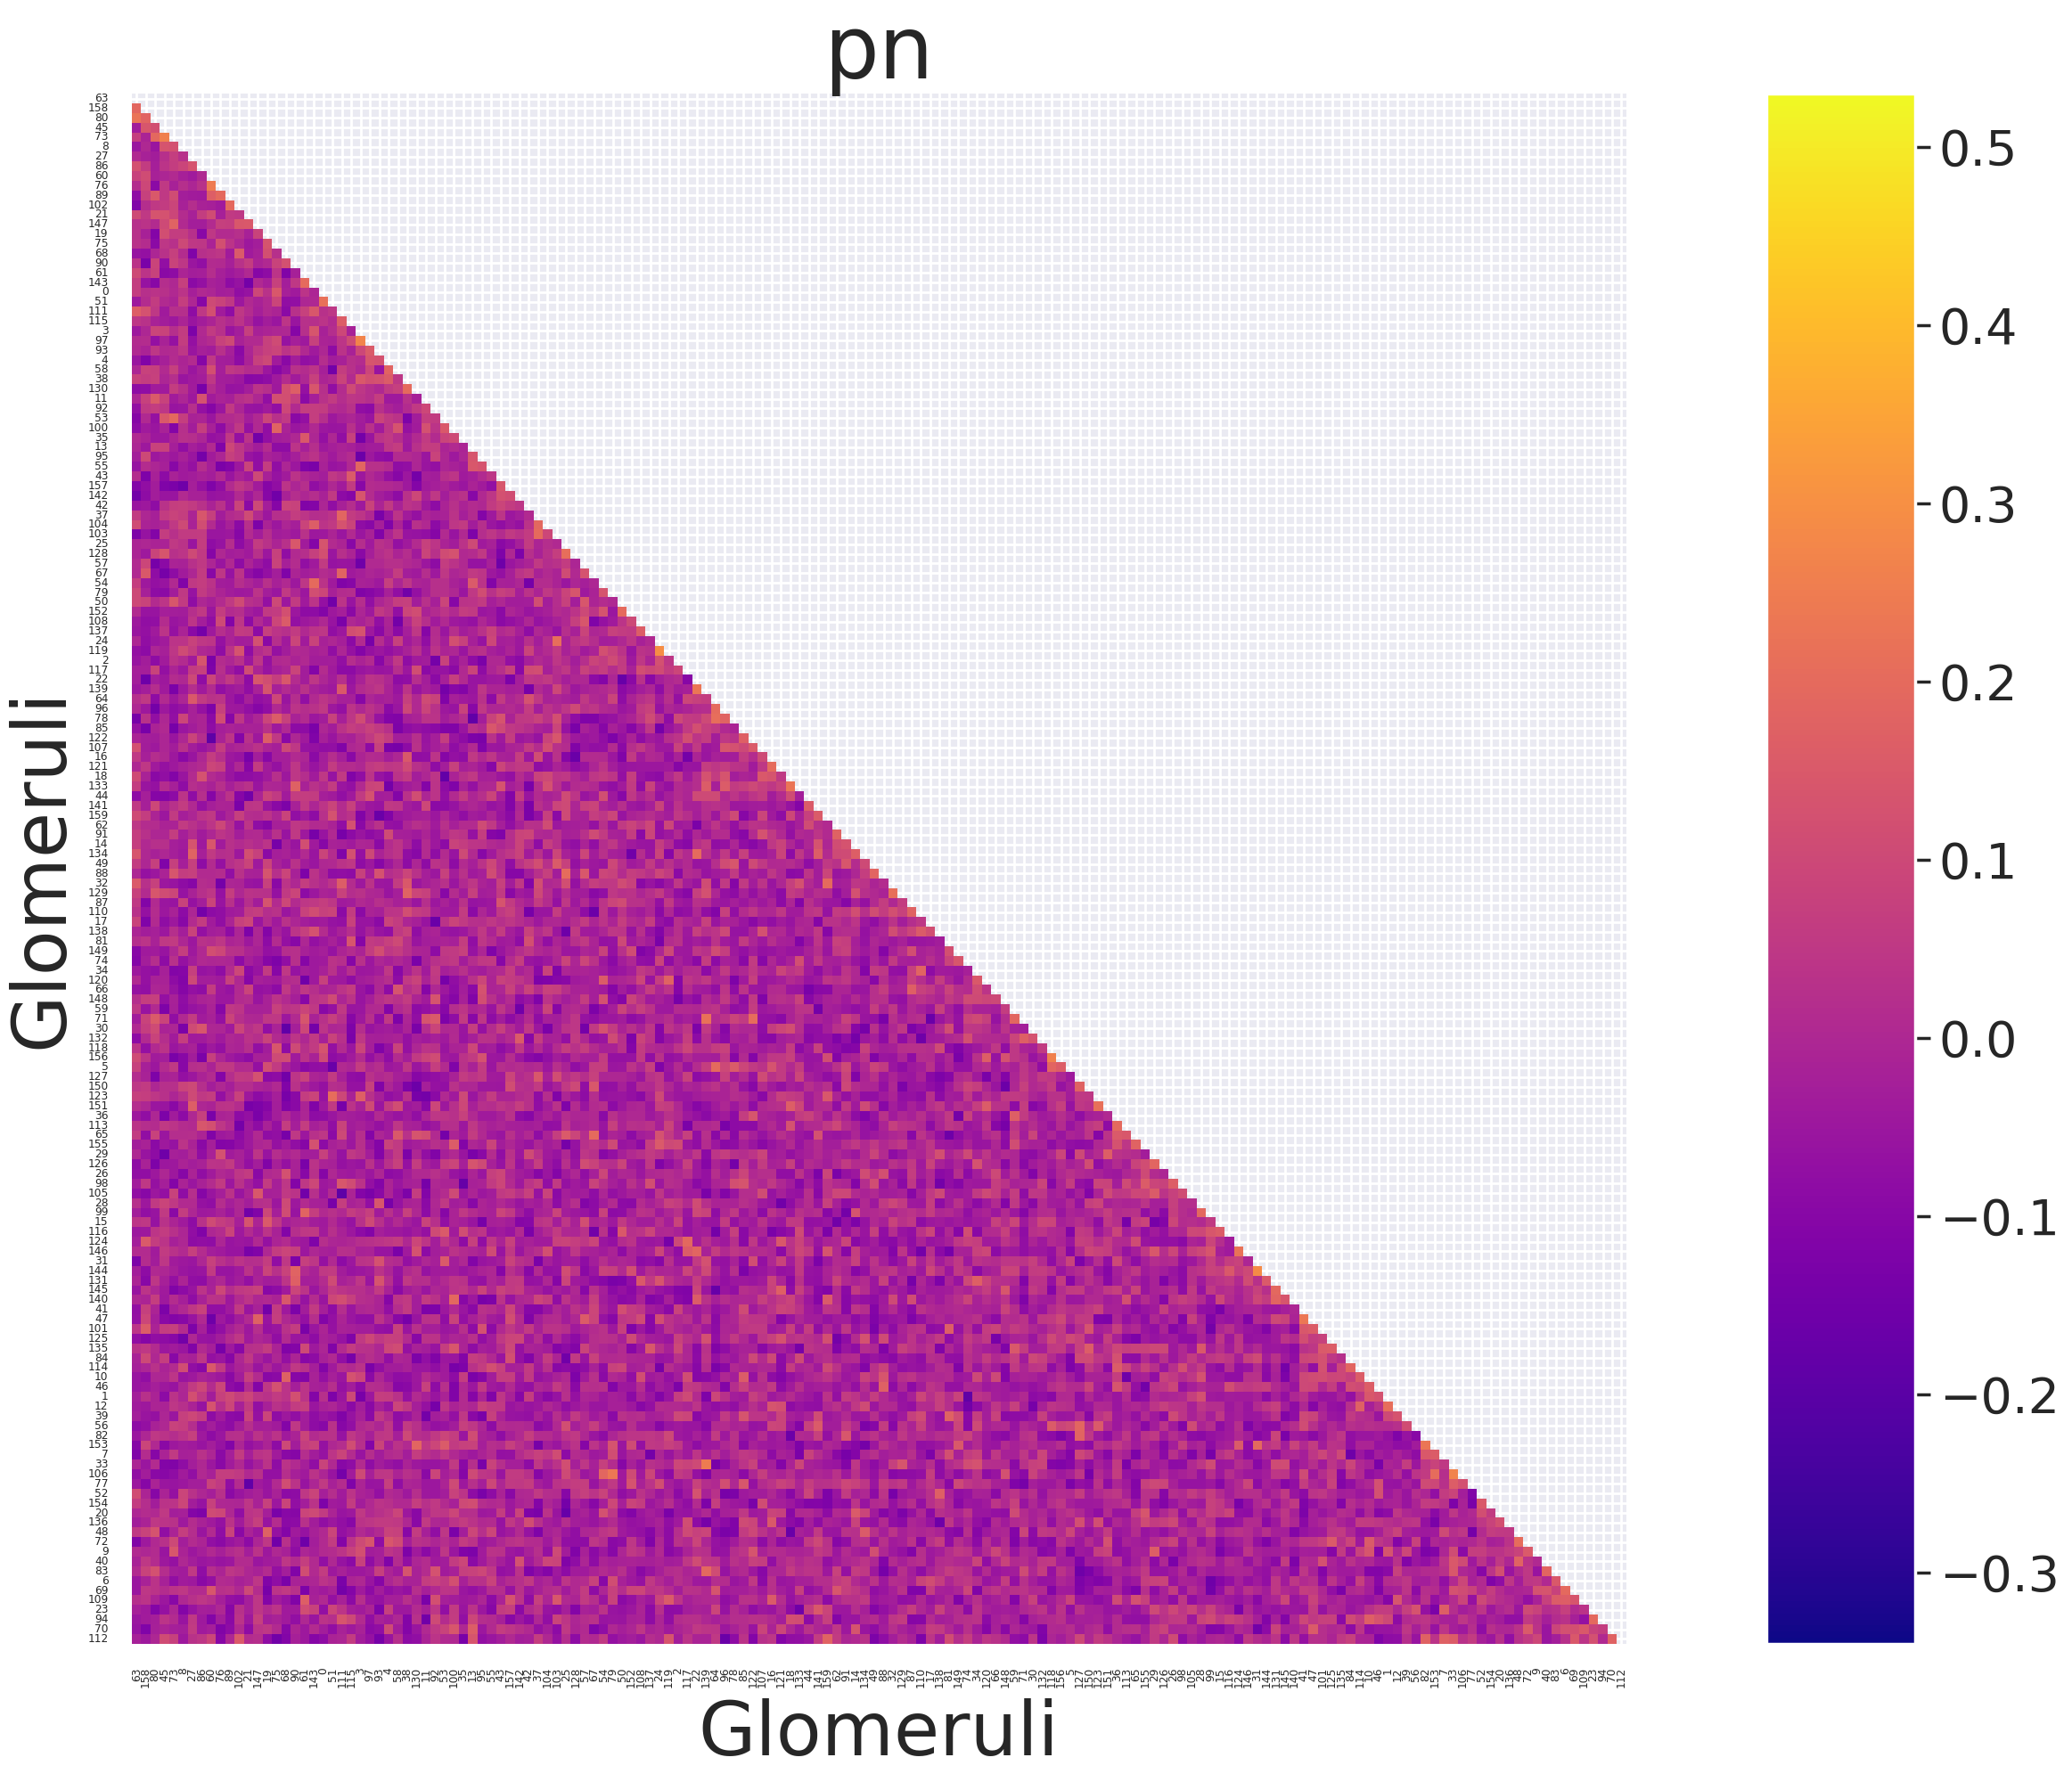
\includegraphics[width=0.8\textwidth]{correlation-awake-no-poisson-pn}
    \caption{Awake without correlated input, average correlation $\overline{Corr_{PN}} = 0.001$}
    \label{fig:awake_state}
  \end{subfigure}
  \begin{subfigure}[t]{0.45\textwidth}
    \centering
    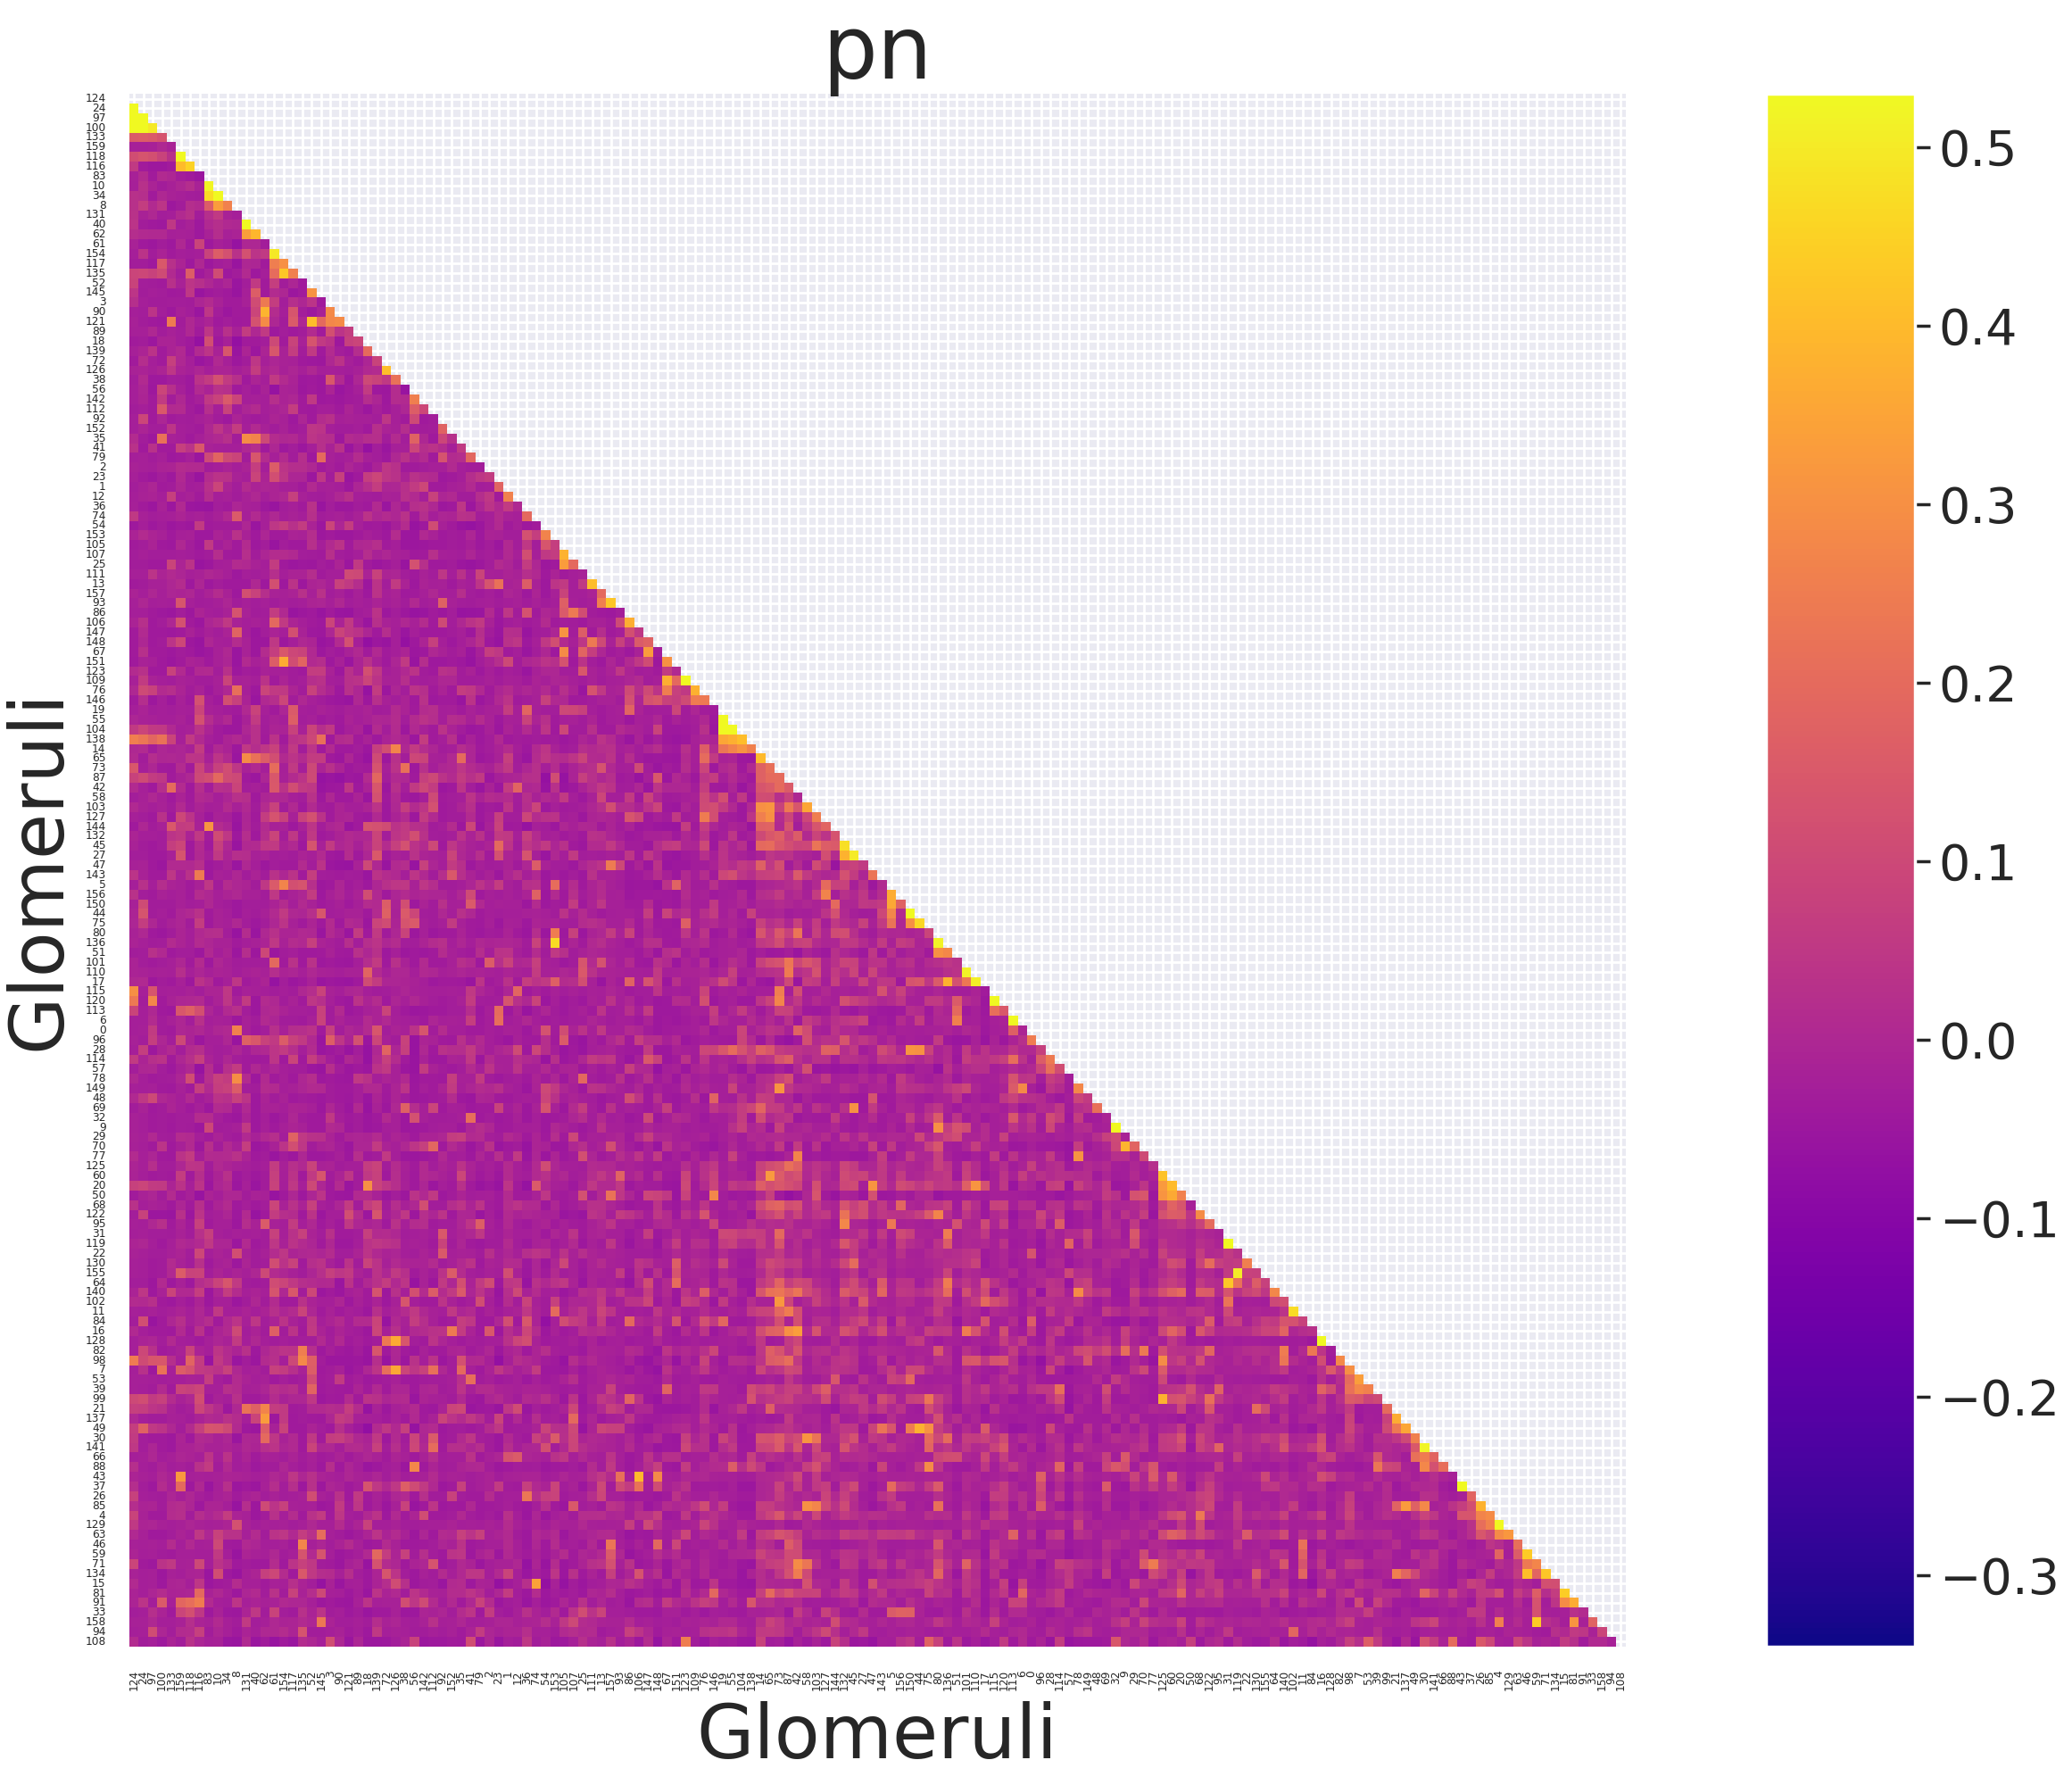
\includegraphics[width=0.8\textwidth]{correlation-awake-poisson-pn}
    \caption{Awake with correlated input, average correlation $\overline{Corr_{PN}} = 0.007$}
    \label{fig:awake_state_with_poisson}
  \end{subfigure}
  \begin{subfigure}[t]{0.45\textwidth}
    \centering
    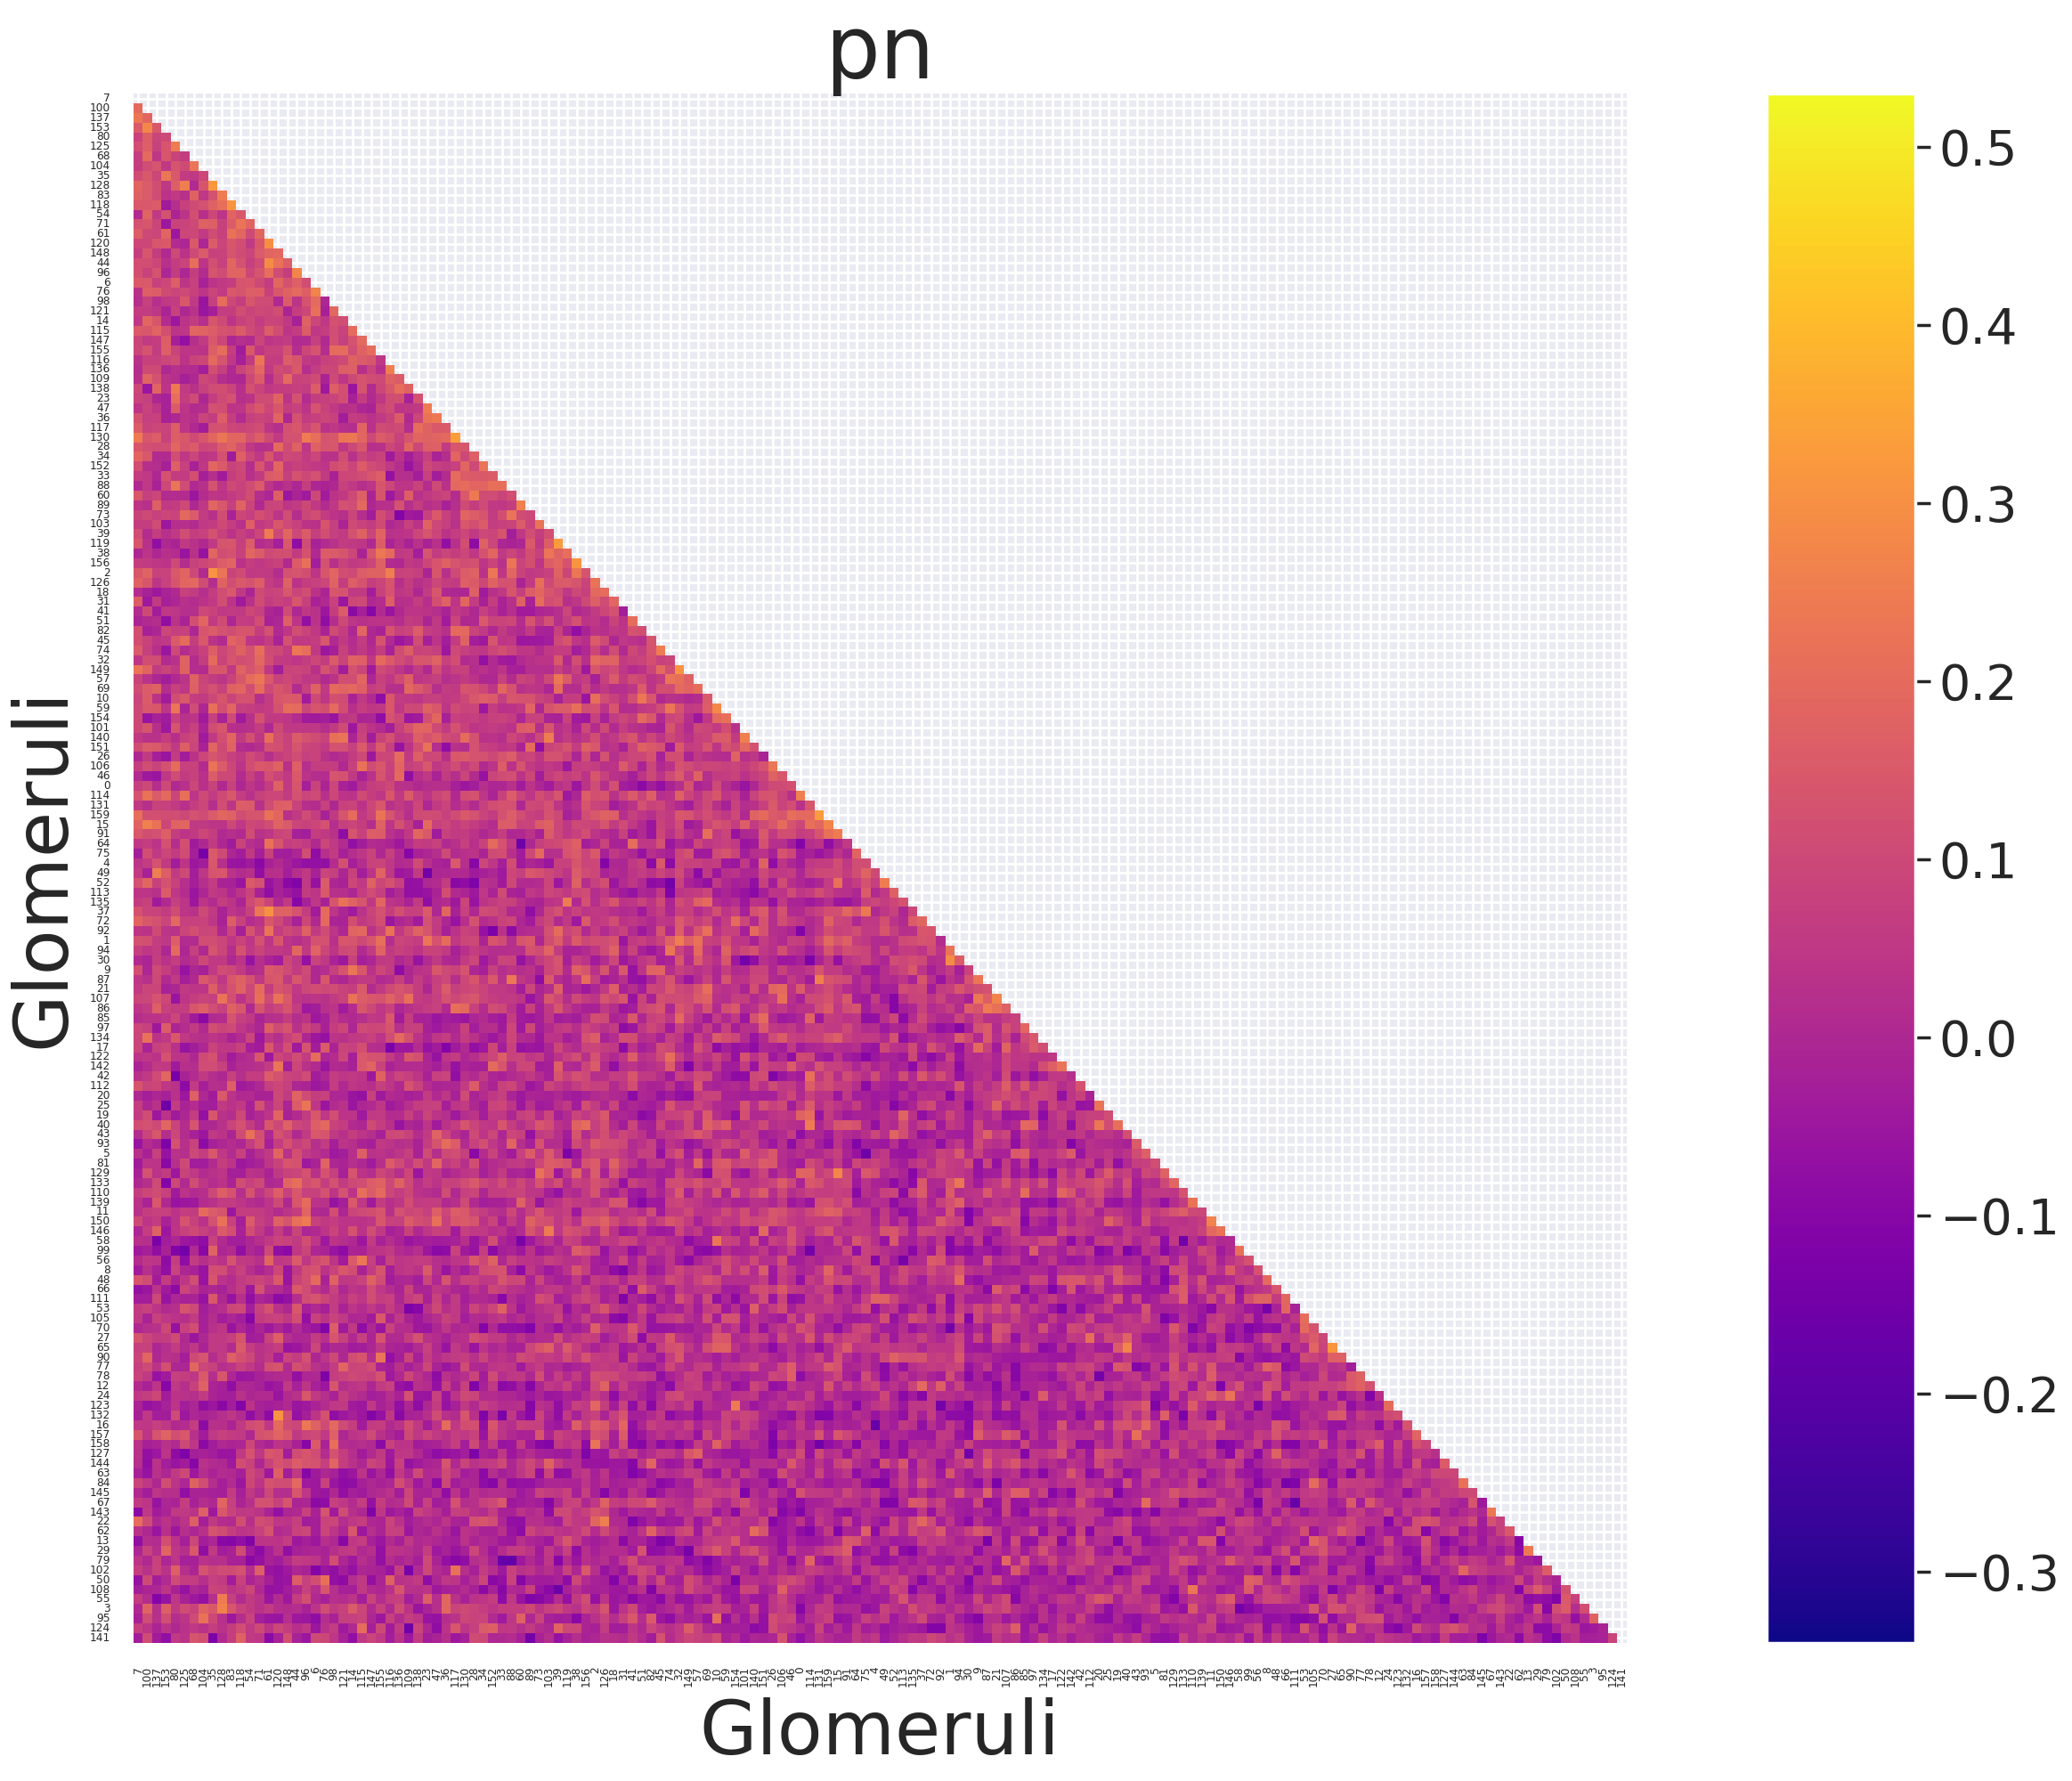
\includegraphics[width=0.8\textwidth]{correlation-halved-poisson-pn}
    \caption{Halved, average correlation $\overline{Corr_{PN}} = 0.01$}
    \label{fig:halved_state}
  \end{subfigure}
  \begin{subfigure}[t]{0.45\textwidth}
    \centering
    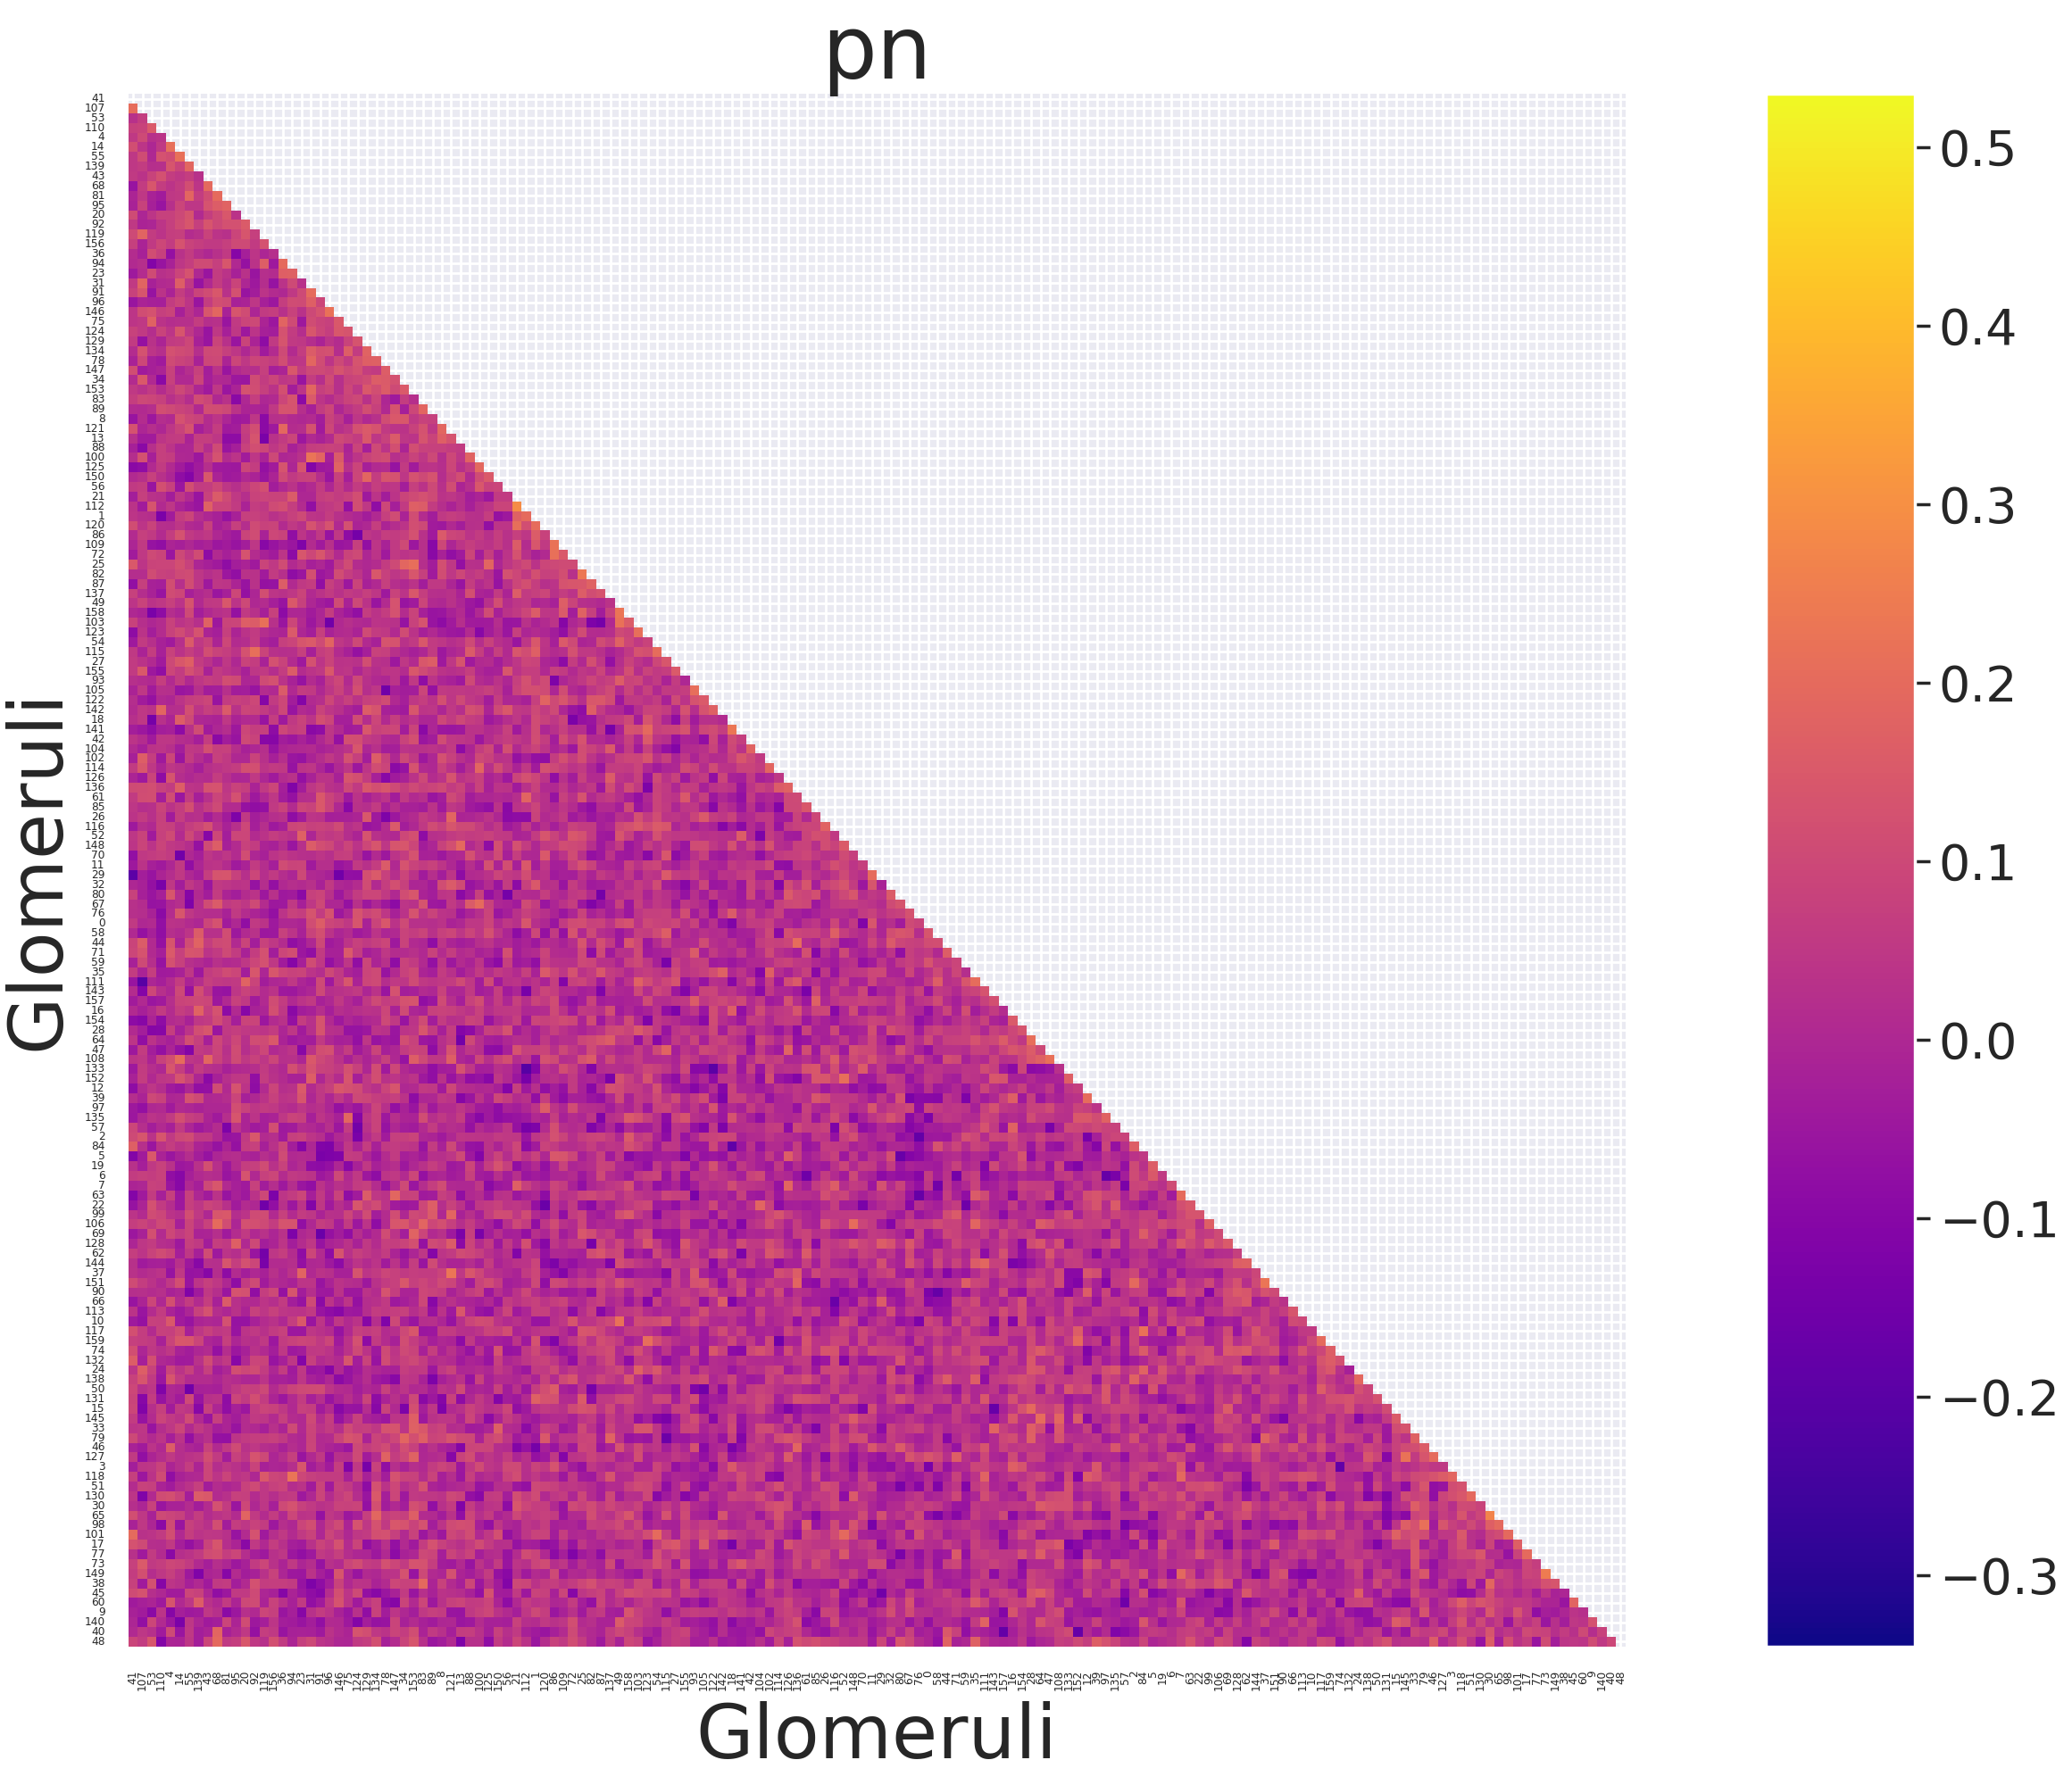
\includegraphics[width=0.8\textwidth]{correlation-quarter-poisson-pn}
    \caption{Quarter, average correlation $\overline{Corr_{PN}} = 0.01$}
    \label{fig:quarter_state}
  \end{subfigure}
  \begin{subfigure}[t]{0.45\textwidth}
    \centering
    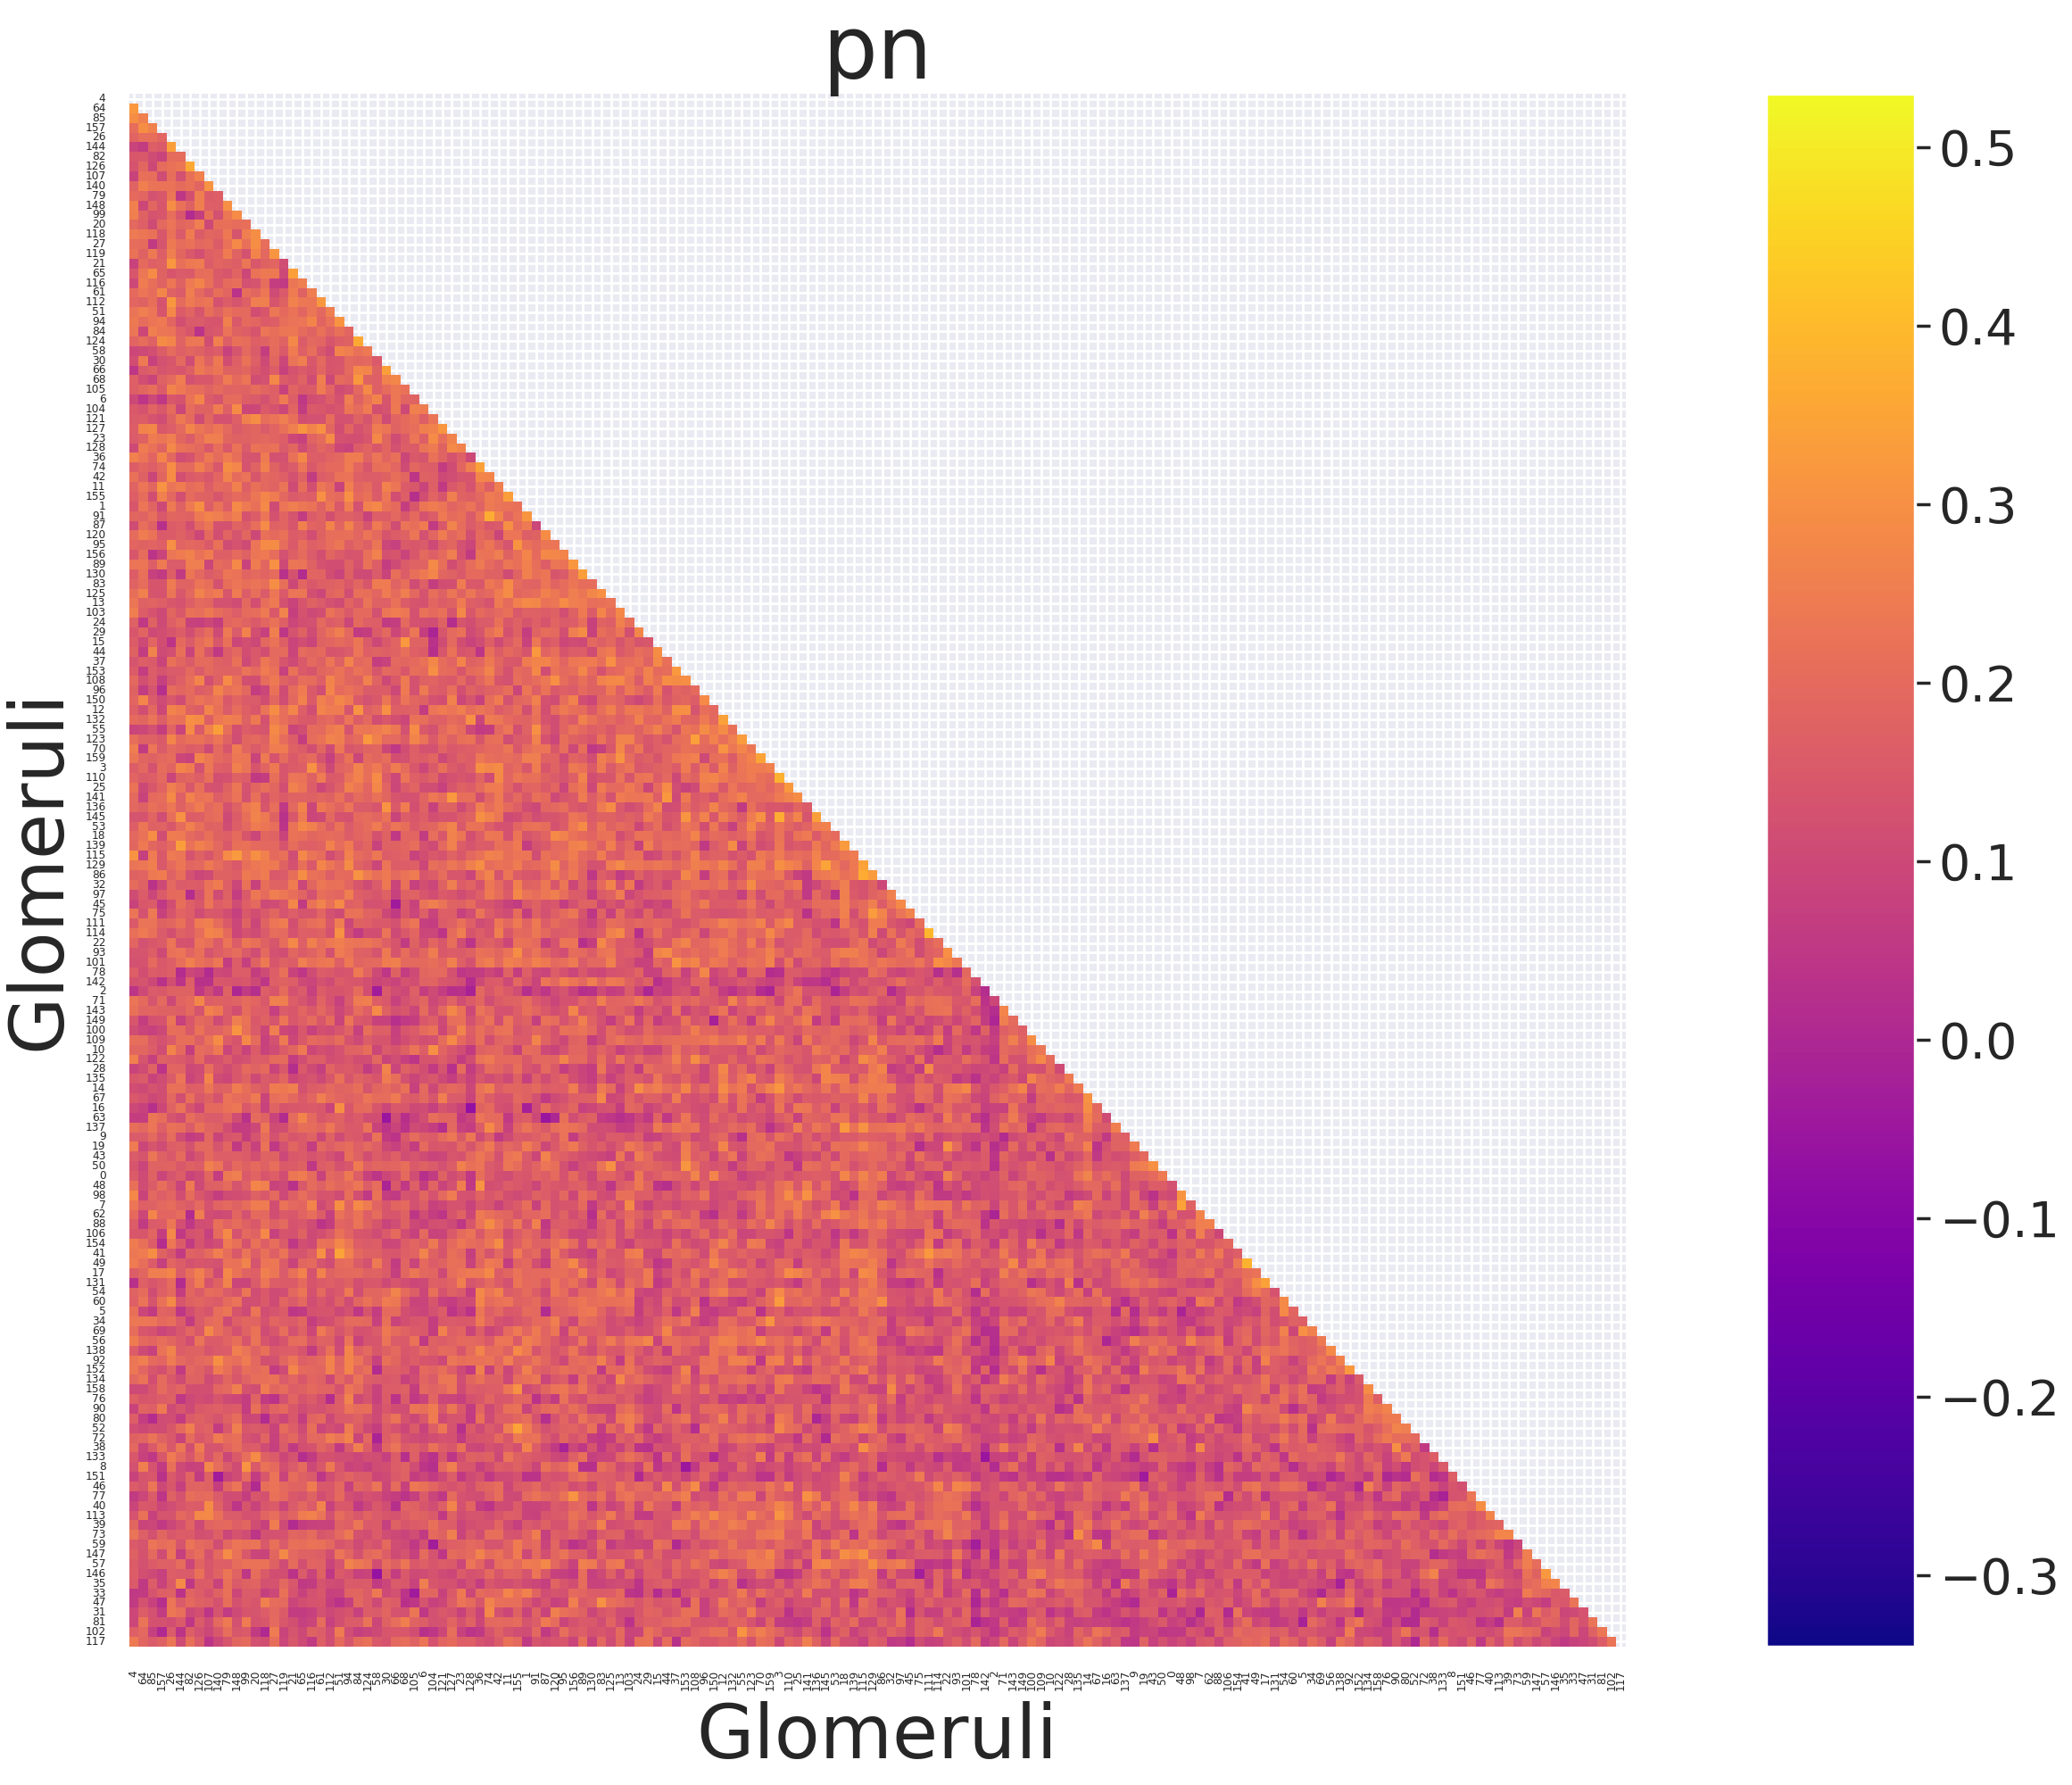
\includegraphics[width=0.8\textwidth]{correlation-tenth-poisson-pn}
    \caption{Tenth, average correlation $\overline{Corr_{PN}} = 0.12$}
    \label{fig:tenth_state}
  \end{subfigure}
  \begin{subfigure}[t]{0.45\textwidth}
    \centering
    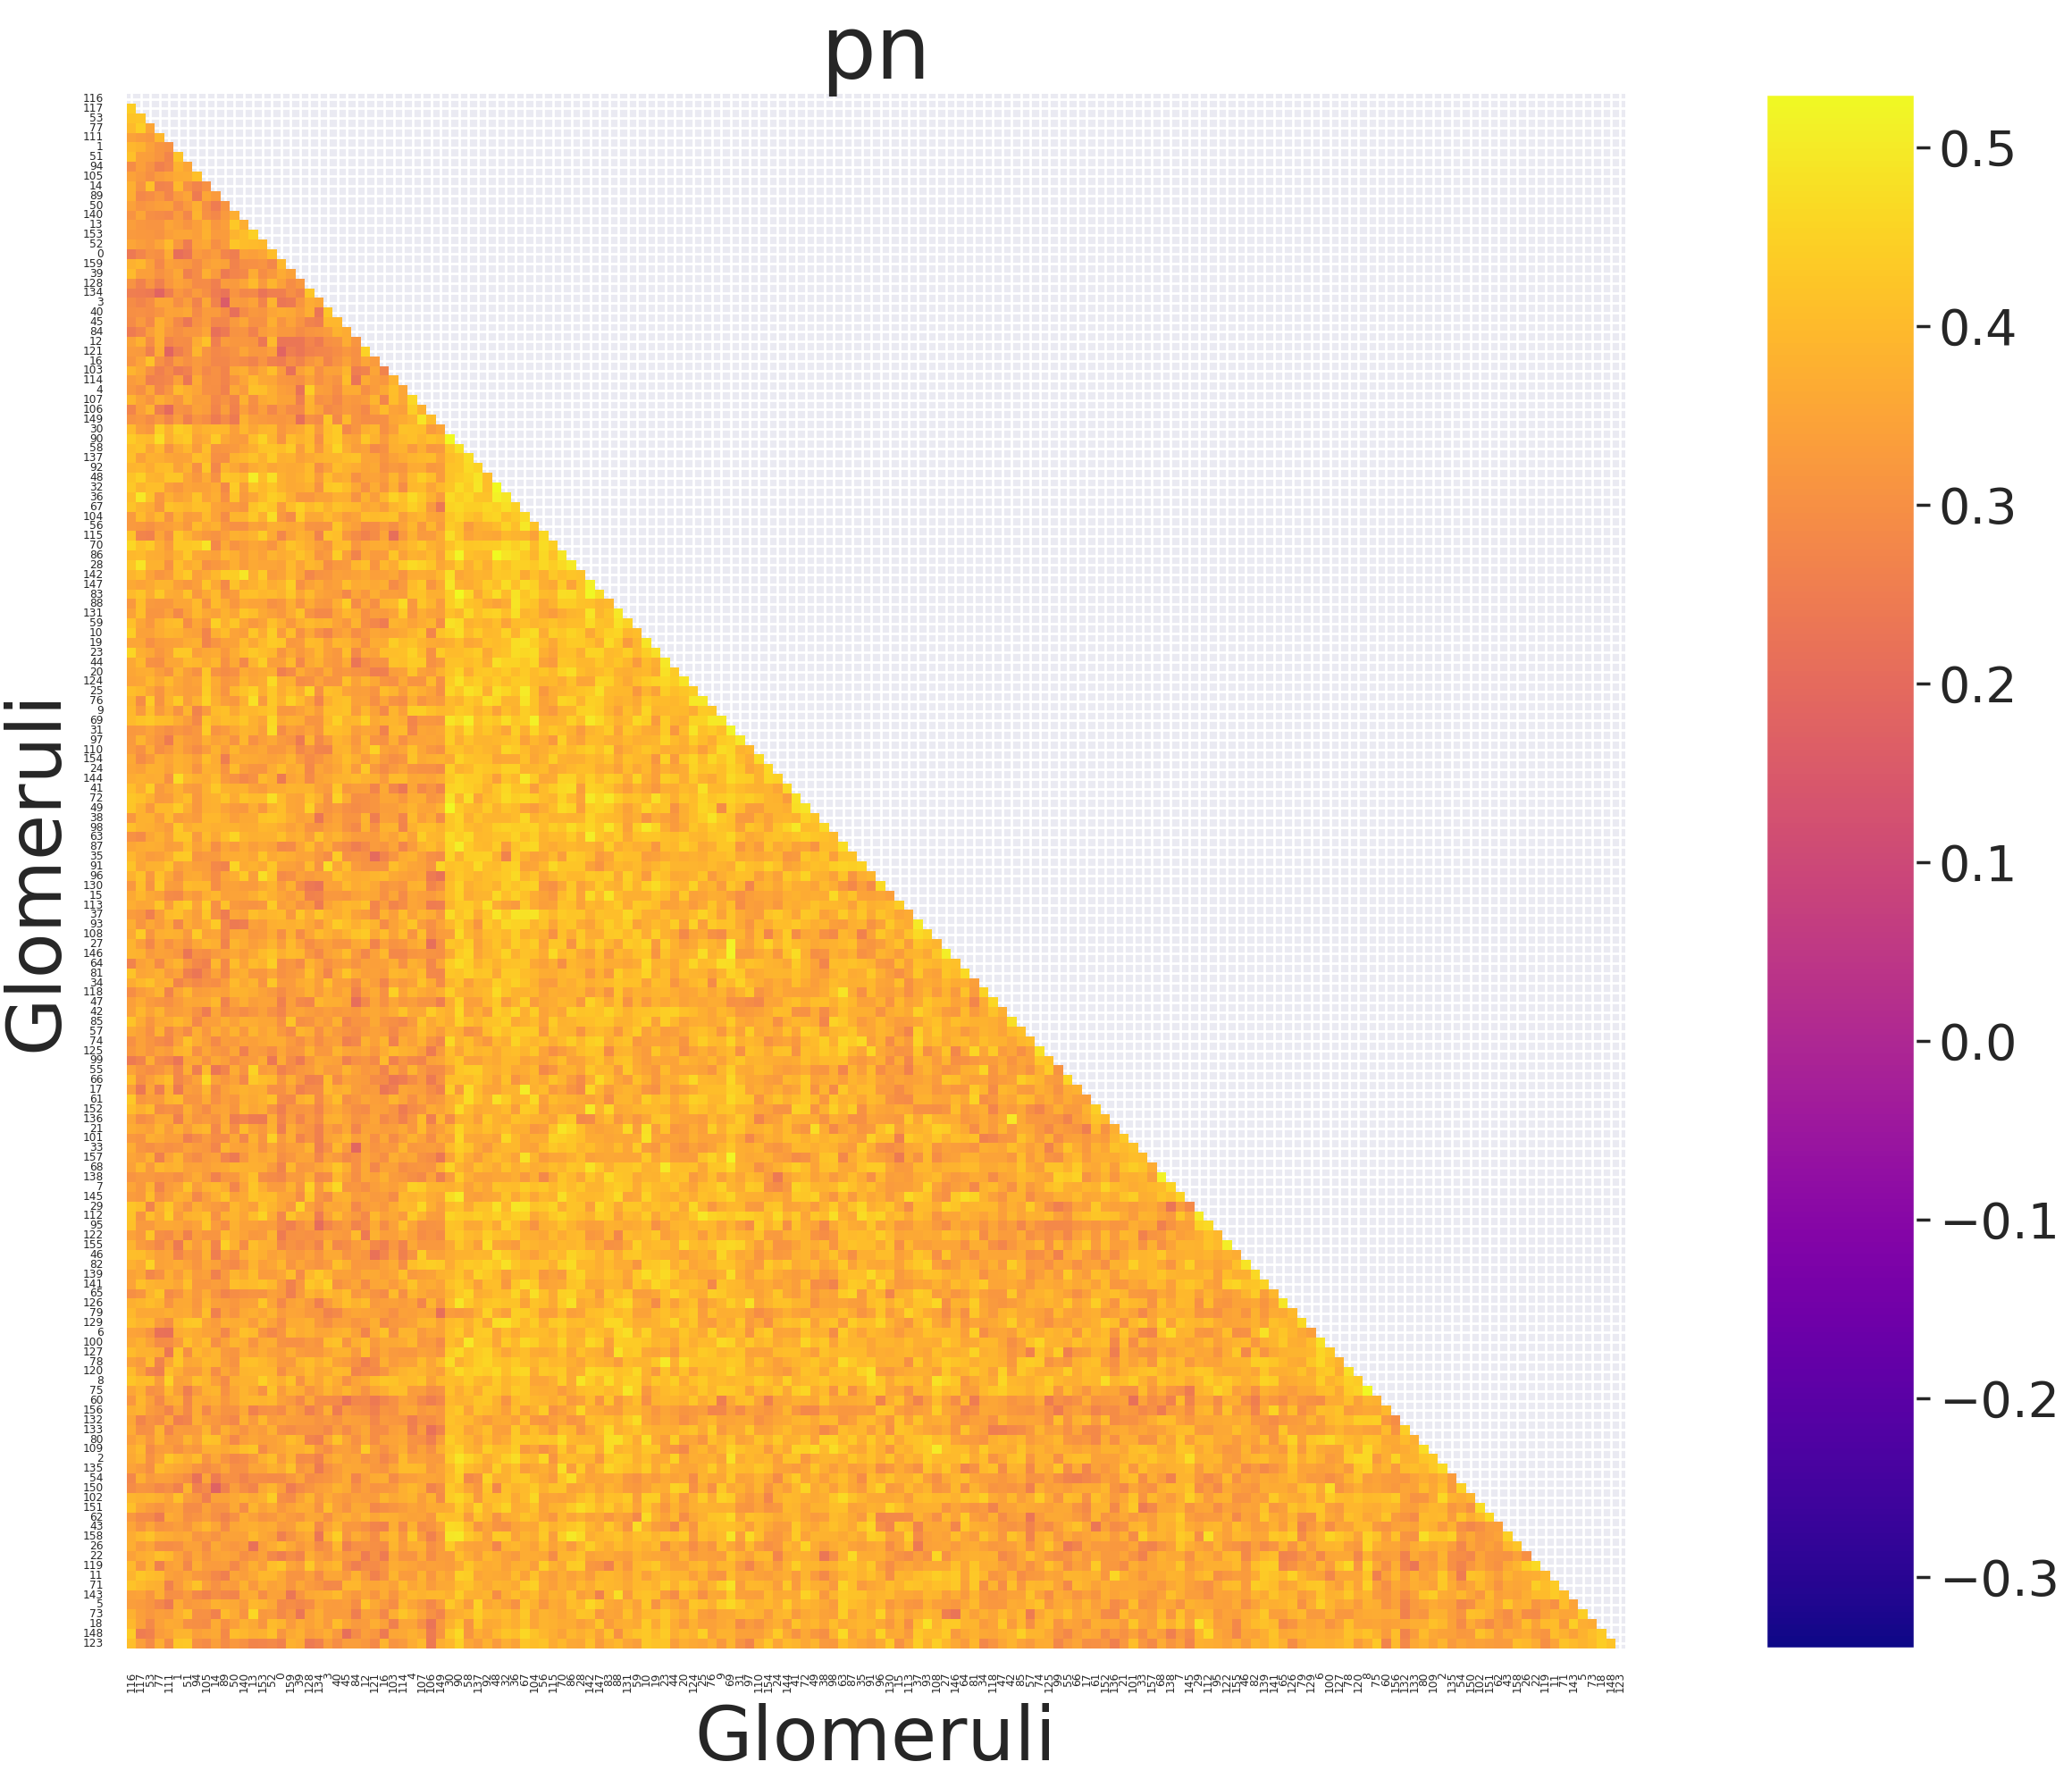
\includegraphics[width=0.8\textwidth]{correlation-hundreth-poisson-pn}
    \caption{Hundredth, average correlation $\overline{Corr_{PN}} = 0.32$}
    \label{fig:hundredth_state}
  \end{subfigure}
  \caption{Correlation between the activity of the projection neurons of the antennal lobe averaged over glomeruli in different conditions. The first row represents the awake state, with and without a correlated input. The successive plots (from left to right and top to bottom) are the same correlation matrices of simulations with increasingly reduced strength of the inhibitory synapses, respectively by a factor of $2$, $4$, $10$ and $100$.}
  \label{fig:correlation_different_conditions}
\end{figure}

  \subsection{Features of the system}
  To further investigate the differences between the awake and asleep state, and to understand what functional properties of the network change in them, several features have been extracted from simulations with different parameters.\\
  These features can be divided into two categories:

  \begin{itemize}
    \item Features related to the spiking activity of the network.
    \item Functional connectivity features.
  \end{itemize}

  Comparing the change in features obtained from simulating the system at different inhibitory synaptic strengths with the feature extracted from an experimental run, further supported the hypothesis that the introduction of a correlated input together with the reduction in inhibitory strength are the mechanisms that contribute to the different pattern of activity between the two states.
  In particular, the simulation that best replicated experimental results is the ``Quarter'' one, where the inhibitory synapses have been reduced by a factor of four.\\
  Interestingly, not all the features change monotonically with the decrease in inhibitory synapses' strength.
  Features concerned with the statistical distribution of the spiking activity of the network, such as:

  \begin{itemize}
    \item Standard deviation (section \ref{sec:std}).
    \item Skewness (section \ref{sec:skewness}).
    \item Kurtosis (section \ref{sec:kurtosis}.
    \item Hurst exponent (section \ref{sec:hurst}).
  \end{itemize}

  Tend to be the only ones that change monotonically.
  All the other features, concerning the functional connectivity of the network tend to show local minima when inhibitory synapses strength is reduced by a factor of two (``Halved'' simulation, figure \ref{fig:halved_state}):

  \begin{itemize}
    \item Efficiency (section \ref{sec:efficiency}).
    \item Sample entropy (section \ref{sec:sampen}).
    \item Degree (section \ref{sec:degree}).
  \end{itemize}

  Or when they are reduced by a factor of four (``Quarter'' simulation, figure \ref{fig:quarter_state}):

  \begin{itemize}
    \item Transitivity (section \ref{sec:transitivity}).
    \item DFA (section \ref{sec:dfa}).
  \end{itemize}

  Local maxima can be found for a reduction factor of four, together with local minima for a reduction factor of two for:

  \begin{itemize}
    \item Frobenius norm (section \ref{sec:norm}).
    \item Betweenness (section \ref{sec:betweenness}).
  \end{itemize}

  All features remain almost unchanged when the reduction factor goes from $10$ to $100$, suggesting that the inhibitory synapse's function is not significant anymore and the reduction is too strong.\\
  The local minima in the ``Halved'' simulation can be explained by the fact that the inhibitory synapses are still strong enough to synchronize the activity of the projection neurons and the introduction of the correlated input changes drastically the inhibition pattern, causing in turn a different conformation of functional connections.
  Local minima in the ``Quarter'' simulation are found in measures that involve the interconnection of the network, suggesting an increase in functional connection for these measures.
  They could be explained by the slight increase in the average correlation neurons in this condition, which even though it could be ascribed to statistical error, has this effect on the measures.\\
  All these measures suggest that the sleep state can be found in a region of the parameter space where the inhibitory synapses are not strong enough to synchronize the activity of the projection neurons, but still strong enough to have a significant effect on the functional connectivity of the network.
  This can be reconducted to a close range around the ``Quarter'' simulation in the parameter space (figure \ref{fig:feature_comparison}).

\begin{figure}
  \centering
  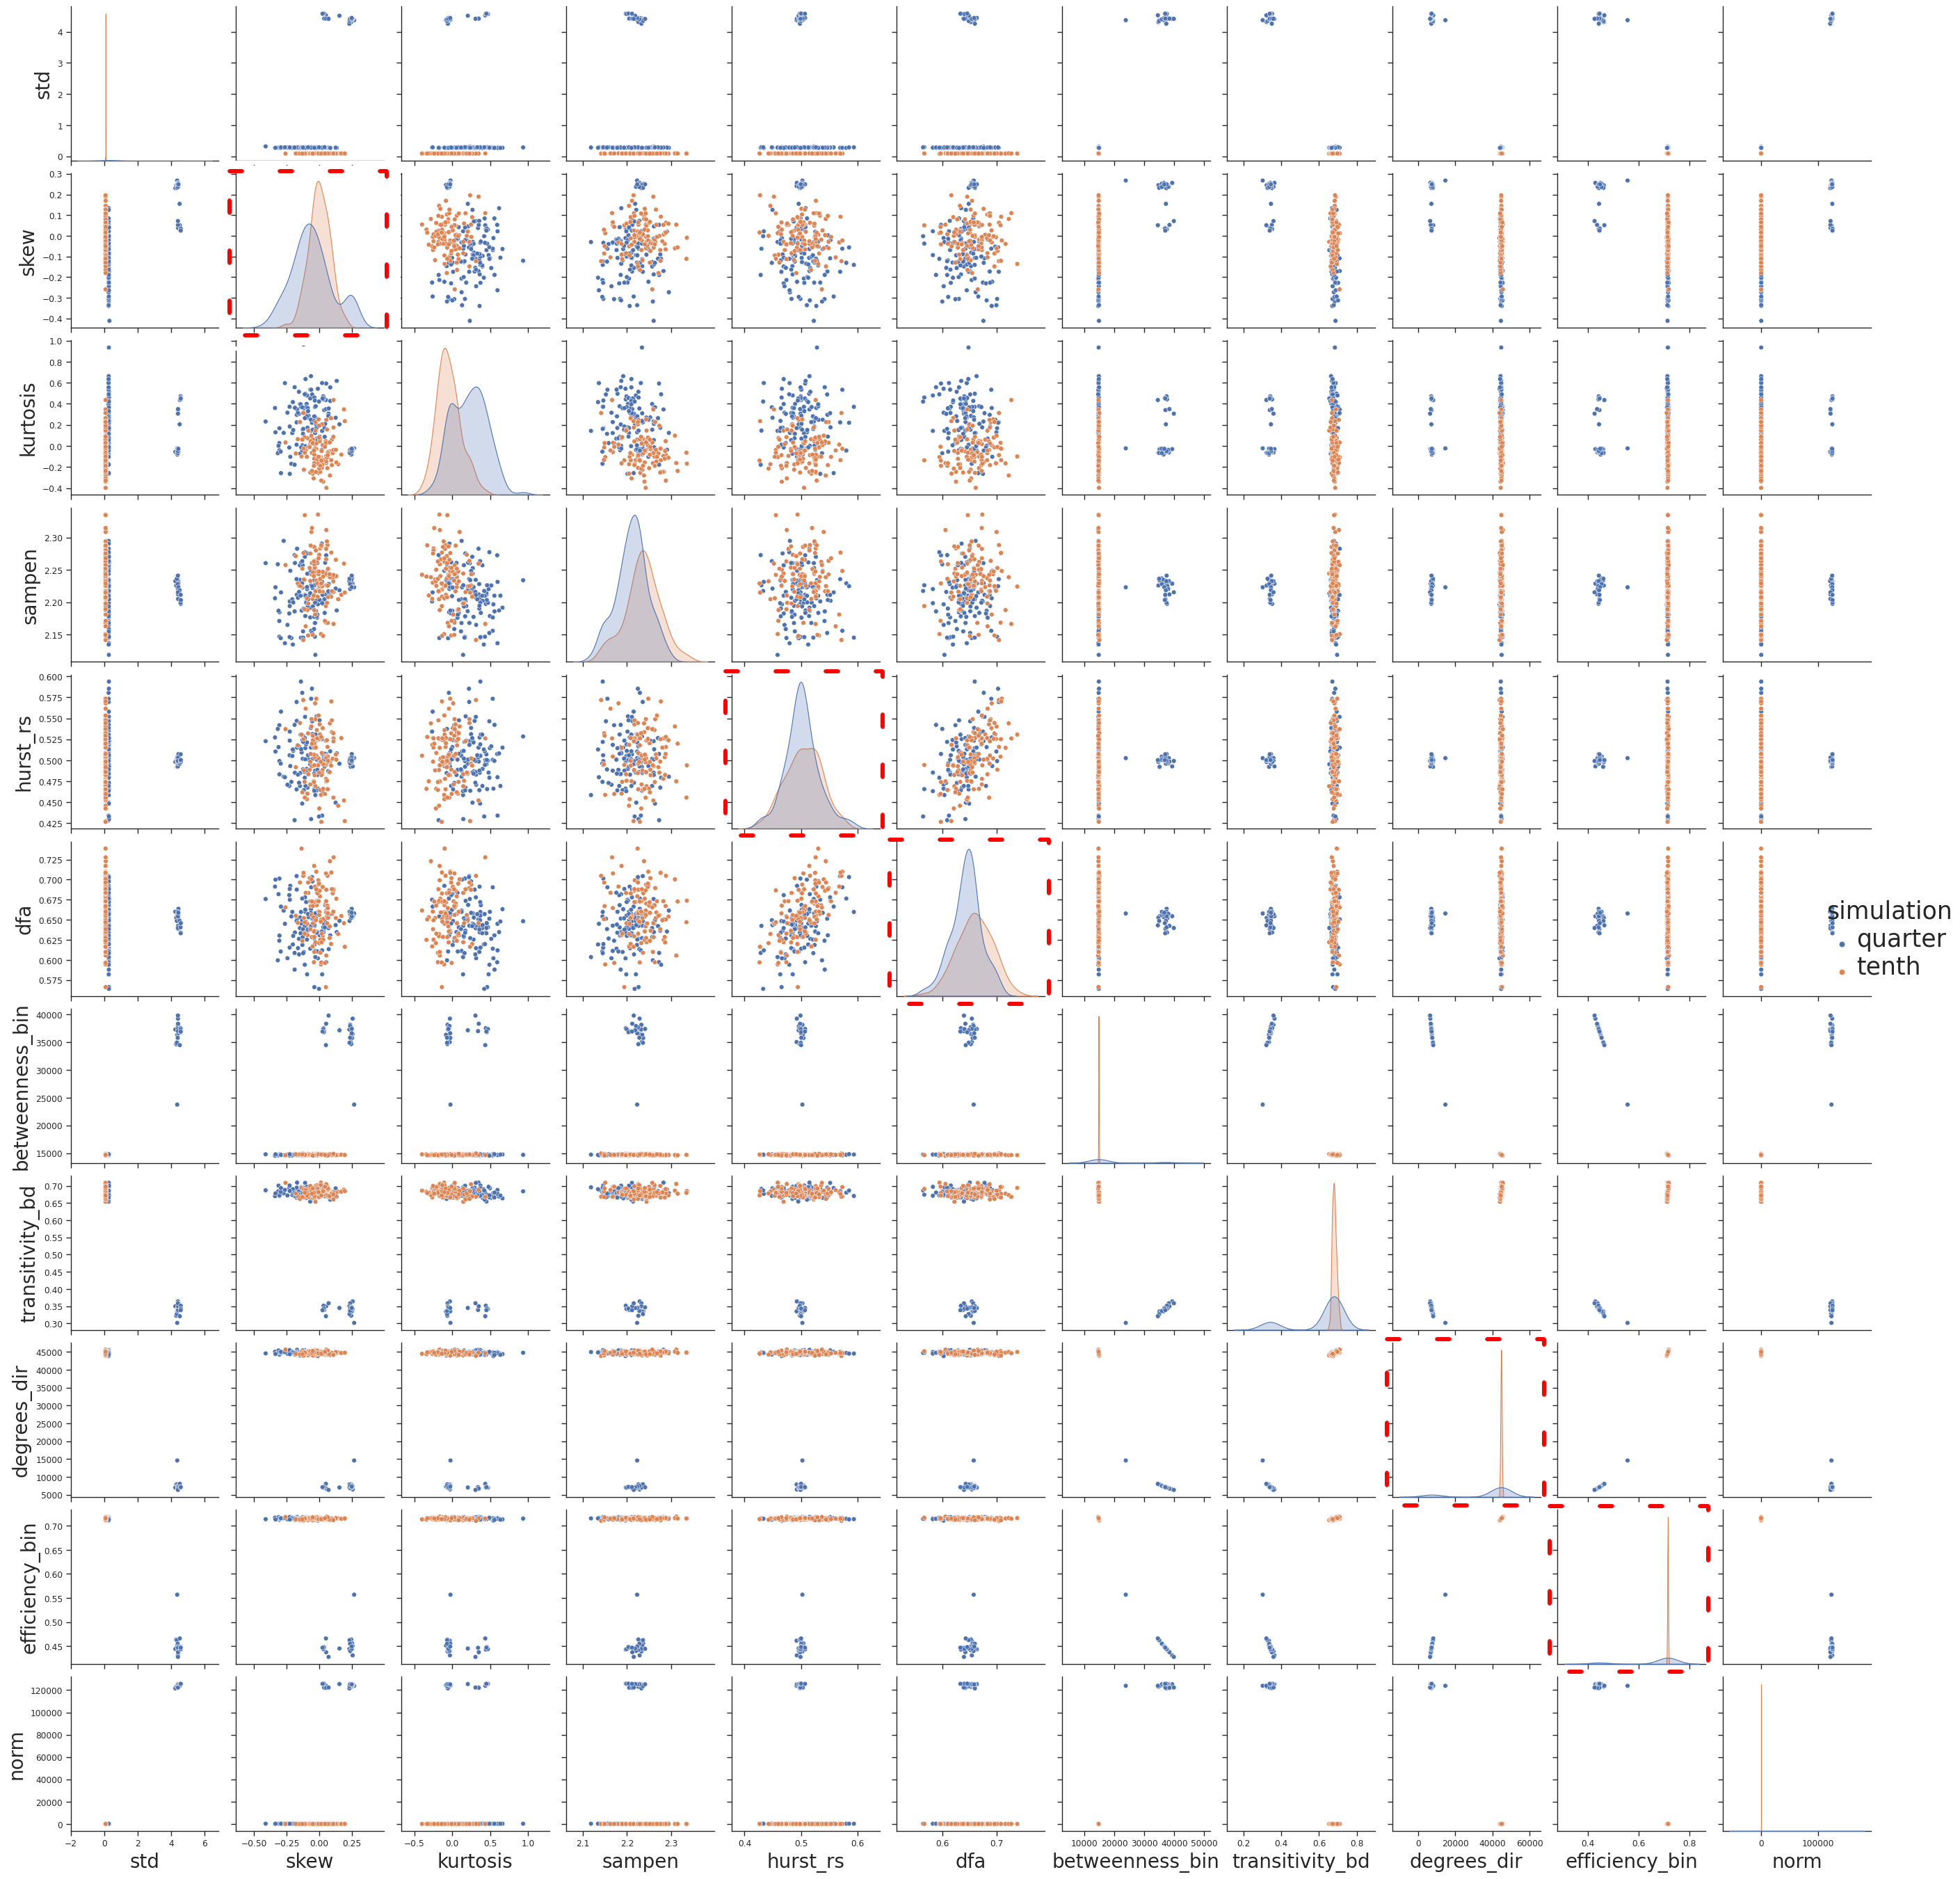
\includegraphics[width=\textwidth]{feature-comparison-quarter-normal}
  \caption{Comparison between the extracted features of the awake condition (in orange) and the putative sleep condition (in blue), features that best fit experimental results are highlighted in red.}
  \label{fig:feature_comparison}
\end{figure}

\section{Putative biological mechanisms}
The results presented here suggest that the differences in activity patterns between the asleep and awake states are due to two major putative mechanisms:

\begin{itemize}
  \item The reduction of inhibitory synapses' strength.
  \item The introduction of a correlated input.
\end{itemize}

Both of these processes can be linked to biological mechanisms that happen both in the honeybee and in the human brain.

  \subsection{Reduction of inhibitory synapses' strength}
  The reduction of inhibitory synapses' strength is a process that happens in the honeybee brain during sleep, and it is thought to have an important role in humans.
  In particular, GABAergic synapses in hippocampal CA1 pyramidal neurons in mice, neurons involved in the memory consolidation and integration processes, undergo daily rhythmic alteration.
  Consistently with electrophysiological data, wake decreased the synaptic expression of $\alpha_1/\alpha_2$-$GABA_ARs$ but increased surface expression of $\alpha_4/\alpha_5$-$GABA_ARs$ in the hippocampus, causing a net decrease in inhibitory synapses' strength.
  This implies a profound difference in the control of neuronal network function across the asleep and awake states.
  Moreover, in human disorders in the GABAergic inhibition mechanisms are linked with insomnia \cite{insomnia}.
  Wakefulness is increased when the ventral midbrain/pons area is chemogenetically inhibited \cite{gaba-ventral}, suggesting that GABAergic neurons have a fundamental role in sleep regulation in mammals.
  Cheomgenetic activation of ventral midbrain/pons GABAergic neurons induces slow-wave-sleep.\\
  Consistently with the results presented here this process in mice is thought to contribute to the increase in correlation of network activity, which is speculated to facilitate memory consolidation during sleep.

  \subsection{Introduction of a correlated input}
  Although no characteristic EEG trace is recorded in the honey bee \cite{sleep-mammals}, global oscillation and neuron grouping are common in humans and mice during slow wave sleep \cite{sws}.
  During slow wave sleep the brain is characterized by a slow oscillation in the range of $\SI{0.5}{\hertz}$, with a high amplitude and a low frequency.
  The neocortex and the hippocampus interact such that neocortical slow oscillations drive the repeated reactivation of newly encoded memories in the hippocampus, driving these representations to become long-term.\\
  The origin of this correlated input is not clear and has not been observed in the antennal lobe of the honey bee, but it is a feature that is able to reproduce observed behavior and is akin to mammals' EEG traces.
  This suggests a global factor that drives the antennal lobe behavior during sleep, without being able to pinpoint its exact origin.
  Putative mechanisms for the increase in spiking synchronization could be attributed to several processes \cite{synchronization-processes}.
  Firstly chemical synaptic transmission of not modelled feedback connections analogous to the mammalian cortico-thalamo-cortical feedback loop, as it has been modeled for the \textit{Drosophila} antenna \cite{model-with-feedback}.
  Gap junctions, or electrical synapses, allow direct flux of ions between connected cells, providing a mechanism of communication that is action potential independent: changes of membrane voltage could in one neuron would trigger current flow between coupled neurons leading to corresponding changes of membrane cells, acting as low-pass filters.
  In cortical networks groups of GABA-releasing interneurons and glial cells are interconnected via gap junctions, suggesting that electrical coupling may occur between axons of pyramidal neurons.
  Lastly, extracellular currents produced by other brain regions constituting local field potentials may directly influence the electrical properties of neurons, causing changes in excitability with a global influence.
